\documentclass[12pt,a4paper]{article}
\usepackage{amsmath, amssymb, geometry, booktabs, xcolor, hyperref,
            listings, pgfplots, tcolorbox, enumitem, fancyhdr, tikz, array}
\geometry{margin=2.5cm}
\pgfplotsset{compat=1.18}
\tcbuselibrary{skins, breakable}

% ----------------------------------------------------------------
% tcolorbox environments  (positional title [1], NOT [1][])
% ----------------------------------------------------------------
\newtcolorbox{curiositybox}[1]{colback=yellow!10, colframe=orange!80!black, fonttitle=\bfseries, title=#1, breakable}
\newtcolorbox{infobox}[1]{colback=blue!5, colframe=blue!60!black, fonttitle=\bfseries, title=#1, breakable}
\newtcolorbox{mistakebox}[1]{colback=red!5, colframe=red!60!black, fonttitle=\bfseries, title=#1, breakable}
\newtcolorbox{learnbox}[1]{colback=green!5, colframe=green!60!black, fonttitle=\bfseries, title=#1, breakable}

% ----------------------------------------------------------------
% lstlisting  (Python)
% ----------------------------------------------------------------
\lstset{language=Python, basicstyle=\ttfamily\small, keywordstyle=\color{blue},
        commentstyle=\color{gray}, stringstyle=\color{red},
        showstringspaces=false, breaklines=true, frame=single}

% ----------------------------------------------------------------
% fancyhdr
% ----------------------------------------------------------------
\pagestyle{fancy}
\fancyhf{}
\lhead{Topic 01: Functions of Complex Variable}
\rhead{Unit I --- Complex Variables}
\cfoot{\thepage}

% ----------------------------------------------------------------
% Title
% ----------------------------------------------------------------
\title{Topic 01: Introduction to Functions of Complex Variable \\
       \large Unit I --- Complex Variable: Differentiation}
\author{JNTUA College of Engineering (Autonomous)}
\date{}

% ================================================================
\begin{document}
% ================================================================

\maketitle
\tableofcontents
\newpage

% ----------------------------------------------------------------
% OPENING HOOK
% ----------------------------------------------------------------
\begin{curiositybox}{Hook}
In real-variable calculus, we input one real number and get one real output.
But what if both the input and output have two parts --- real and imaginary?
Suddenly, a function does not just draw a curve; it can transform an entire
plane.  That is the world of complex variables.
\end{curiositybox}

% ================================================================
\section{Why This Topic Matters}
% ================================================================

Engineering mathematics reaches a new level of power once we step beyond the
real line and work in the complex plane.  Problems in signal processing,
fluid dynamics, electromagnetic theory, and control systems all become
cleaner and more tractable using complex-variable methods.

\begin{center}
\begin{tabular}{>{\bfseries}p{6.5cm} p{6.5cm}}
\toprule
If we stop at real functions \ldots & What complex functions allow us to do \\
\midrule
We can only model phenomena on a line or in a plane with two real equations.
& One complex equation replaces two real equations, halving the bookkeeping. \\
\addlinespace
Solving Laplace's equation in 2-D requires special tricks.
& Analytic functions automatically satisfy Laplace's equation --- conformal
  mapping solves boundary-value problems elegantly. \\
\addlinespace
Fourier and Laplace transforms need ad hoc justification.
& They emerge naturally as special contour integrals in the complex plane. \\
\addlinespace
Circuit analysis for AC signals uses awkward real trigonometry.
& Phasor notation \(V = V_0 e^{i\omega t}\) makes AC calculations immediate. \\
\addlinespace
Computing certain real definite integrals requires ingenuity.
& The Residue Theorem evaluates them in a few systematic steps. \\
\bottomrule
\end{tabular}
\end{center}

\begin{learnbox}{Key Takeaway}
Mastering complex variables is not merely an academic exercise --- it is the
language in which electrical engineering, fluid mechanics, and quantum
mechanics are most naturally written.
\end{learnbox}

% ================================================================
\section{Recap of Complex Numbers}
% ================================================================

\begin{infobox}{Definition --- Complex Number}
A \textbf{complex number} is an ordered pair of real numbers written as
\[
  z = x + iy, \quad x,y \in \mathbb{R},\quad i = \sqrt{-1}.
\]
\begin{itemize}[noitemsep]
  \item \textbf{Real part}: \(\operatorname{Re}(z) = x\)
  \item \textbf{Imaginary part}: \(\operatorname{Im}(z) = y\)
        \quad (note: the imaginary part is \(y\), \emph{not} \(iy\))
  \item \textbf{Equality}: \(x_1+iy_1 = x_2+iy_2 \iff x_1=x_2\) and
        \(y_1=y_2\)
  \item \textbf{Addition}: \((x_1+iy_1)+(x_2+iy_2)=(x_1+x_2)+i(y_1+y_2)\)
  \item \textbf{Subtraction}: \((x_1+iy_1)-(x_2+iy_2)=(x_1-x_2)+i(y_1-y_2)\)
  \item \textbf{Multiplication}:
        \((x_1+iy_1)(x_2+iy_2)=(x_1 x_2 - y_1 y_2)+i(x_1 y_2+x_2 y_1)\)
  \item \textbf{Complex conjugate}: \(\overline{z} = x - iy\)
  \item \textbf{Modulus}: \(|z| = \sqrt{x^2+y^2}\)
  \item \textbf{Amplitude (argument)}: \(\arg(z) = \theta\) where
        \(\tan\theta = y/x\), principal value \(\theta \in (-\pi,\pi]\)
  \item \textbf{Polar form}:
        \(z = r(\cos\theta + i\sin\theta) = re^{i\theta}\), \quad \(r=|z|\)
\end{itemize}
\end{infobox}

\subsection*{Worked Example 2.1 --- Basic operations}

Let \(z_1 = 3+4i\) and \(z_2 = 1-2i\).  Find the sum, difference, product,
and modulus of each.

\textbf{Sum:}
\[
  z_1 + z_2 = (3+1)+i(4+(-2)) = 4+2i.
\]

\textbf{Difference:}
\[
  z_1 - z_2 = (3-1)+i(4-(-2)) = 2+6i.
\]

\textbf{Product:}
\[
  z_1 z_2 = (3)(1)-(4)(-2) + i\bigl[(3)(-2)+(4)(1)\bigr]
           = 3+8 + i(-6+4) = 11-2i.
\]

\textbf{Moduli:}
\[
  |z_1| = \sqrt{9+16} = 5, \qquad |z_2| = \sqrt{1+4} = \sqrt{5}.
\]

\begin{learnbox}{Takeaway 2.1}
Always expand \((x+iy)(a+ib)\) using FOIL and replace \(i^2\) by \(-1\)
immediately.  Keep real and imaginary parts clearly separated.
\end{learnbox}

\subsection*{Worked Example 2.2 --- Polar form}

Convert \(z = -1 + i\sqrt{3}\) to polar form.

\[
  r = |z| = \sqrt{(-1)^2+(\sqrt{3})^2} = \sqrt{1+3} = 2.
\]
\[
  \theta = \arg(z).
  \quad \text{Since } x<0,\, y>0 \text{ (second quadrant):}
  \quad \theta = \pi - \arctan\!\left(\frac{\sqrt{3}}{1}\right)
               = \pi - \frac{\pi}{3} = \frac{2\pi}{3}.
\]
\[
  \therefore\; z = 2\!\left(\cos\frac{2\pi}{3} + i\sin\frac{2\pi}{3}\right)
               = 2e^{i2\pi/3}.
\]

\begin{learnbox}{Takeaway 2.2}
Always determine the quadrant of \(z\) before computing \(\arg(z)\).
The formula \(\arctan(y/x)\) alone gives the correct angle only when
\(x > 0\).
\end{learnbox}

% ================================================================
\section{Argand Plane}
% ================================================================

A complex number \(z = x+iy\) can be represented as the point
\((x,y)\) in the Cartesian plane.  When the horizontal axis represents
\(\operatorname{Re}(z)\) and the vertical axis represents
\(\operatorname{Im}(z)\), the plane is called the \textbf{Argand plane}
(or complex plane).  The modulus \(|z|\) is the distance of the point from
the origin, and \(\arg(z)\) is the angle measured counter-clockwise from the
positive real axis.

\begin{infobox}{Key Formulas for the Argand Plane}
\[
  |z| = \sqrt{x^2+y^2}, \qquad
  \arg(z) = \operatorname{Arg}(z)+2k\pi,\quad k\in\mathbb{Z}.
\]
\[
  x = r\cos\theta,\quad y = r\sin\theta,\quad
  z + \overline{z} = 2x,\quad z - \overline{z} = 2iy,\quad
  z\overline{z} = |z|^2.
\]
\end{infobox}

\subsection*{Argand Plane Diagram}

\begin{center}
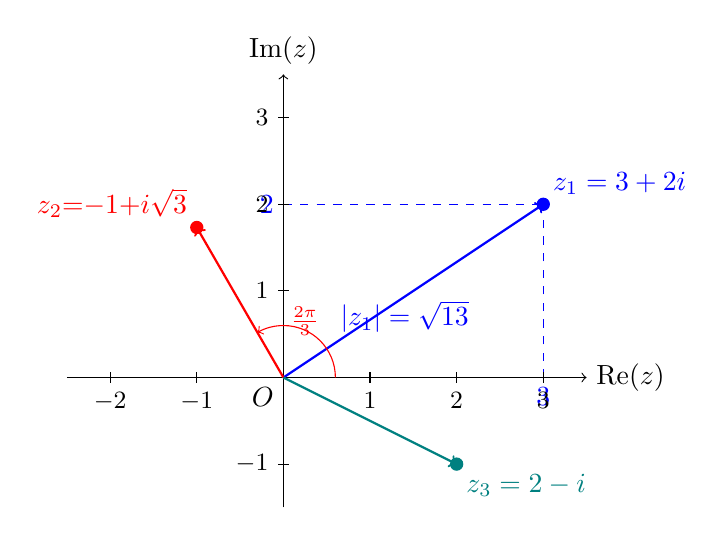
\begin{tikzpicture}[scale=1.1]
  % Axes
  \draw[->] (-2.5,0) -- (3.5,0) node[right] {$\operatorname{Re}(z)$};
  \draw[->] (0,-1.5) -- (0,3.5) node[above] {$\operatorname{Im}(z)$};
  % Origin label
  \node[below left] at (0,0) {$O$};
  % Point z1 = 3 + 2i
  \filldraw[blue] (3,2) circle (2pt) node[above right] {$z_1=3+2i$};
  \draw[blue, dashed] (3,0) node[below] {$3$} -- (3,2);
  \draw[blue, dashed] (0,2) node[left]  {$2$} -- (3,2);
  % modulus arrow for z1
  \draw[blue, thick, ->] (0,0) -- (3,2);
  \node[blue] at (1.4,0.7) {$|z_1|=\sqrt{13}$};
  % Point z2 = -1 + 1.732i
  \filldraw[red] (-1,1.732) circle (2pt)
      node[above left] {$z_2{=}{-1{+}i\sqrt{3}}$};
  \draw[red, thick, ->] (0,0) -- (-1,1.732);
  % angle arc for z2
  \draw[red, ->] (0.6,0) arc[start angle=0, end angle=120, radius=0.6];
  \node[red] at (0.25,0.65) {\small $\frac{2\pi}{3}$};
  % Point z3 = 2 - 1i
  \filldraw[teal] (2,-1) circle (2pt) node[below right] {$z_3=2-i$};
  \draw[teal, thick, ->] (0,0) -- (2,-1);
  % Axis tick marks
  \foreach \x in {-2,-1,1,2,3}
      \draw (\x,0.06) -- (\x,-0.06) node[below] {\small $\x$};
  \foreach \y in {-1,1,2,3}
      \draw (0.06,\y) -- (-0.06,\y) node[left] {\small $\y$};
\end{tikzpicture}
\end{center}

\begin{learnbox}{Takeaway 3.1}
Every complex number is a \emph{point} in the Argand plane.  Addition of
complex numbers corresponds to vector addition; modulus is the length of the
position vector.
\end{learnbox}

% ================================================================
\section{Functions of a Complex Variable}
% ================================================================

\begin{infobox}{Definition --- Complex Function}
A \textbf{function of a complex variable} is a rule \(f\) that assigns to
each \(z = x+iy\) in some domain \(D \subseteq \mathbb{C}\) a complex
number \(w\):
\[
  w = f(z) = u(x,y) + i\,v(x,y),
\]
where \(u(x,y) = \operatorname{Re}(f(z))\) and
\(v(x,y) = \operatorname{Im}(f(z))\) are real-valued functions of two real
variables.
\end{infobox}

Thus, one complex function is \emph{equivalent to} two real-valued functions
\(u\) and \(v\).  This correspondence is central to all of complex analysis.

\subsection*{Worked Example 4.1 --- \(f(z) = z^2\)}

\[
  f(z) = z^2 = (x+iy)^2 = x^2 + 2xyi + i^2 y^2 = (x^2-y^2)+i(2xy).
\]
\[
  \therefore\; u(x,y) = x^2 - y^2, \qquad v(x,y) = 2xy.
\]

\begin{learnbox}{Takeaway 4.1}
Expand using algebra, replace \(i^2=-1\), then collect real and imaginary
parts to identify \(u\) and \(v\).
\end{learnbox}

\subsection*{Worked Example 4.2 --- \(f(z) = z + 1/z\)}

For \(z \neq 0\):
\[
  \frac{1}{z} = \frac{\overline{z}}{|z|^2} = \frac{x-iy}{x^2+y^2}.
\]
\[
  f(z) = x+iy + \frac{x-iy}{x^2+y^2}
       = \left(x + \frac{x}{x^2+y^2}\right)
         + i\left(y - \frac{y}{x^2+y^2}\right).
\]
\[
  u(x,y) = x\!\left(1+\frac{1}{x^2+y^2}\right), \qquad
  v(x,y) = y\!\left(1-\frac{1}{x^2+y^2}\right).
\]

\begin{learnbox}{Takeaway 4.2}
To separate \(1/z\), multiply numerator and denominator by \(\overline{z}\)
and use \(z\overline{z}=|z|^2\).
\end{learnbox}

\subsection*{Worked Example 4.3 --- \(f(z) = e^z\) (introductory)}

\[
  e^z = e^{x+iy} = e^x \cdot e^{iy} = e^x(\cos y + i\sin y).
\]
\[
  u(x,y) = e^x \cos y, \qquad v(x,y) = e^x \sin y.
\]

\begin{learnbox}{Takeaway 4.3}
The complex exponential is defined by \(e^{iy}=\cos y+i\sin y\)
(Euler's formula).  Its real and imaginary parts involve \emph{both}
\(x\) and \(y\).
\end{learnbox}

% ================================================================
\section{Standard Transformations / Mapping Idea}
% ================================================================

A complex function \(w = f(z)\) maps points in the \(z\)-plane
(\(Oxy\)-plane) to points in the \(w\)-plane (\(Ouv\)-plane).  Even simple
functions produce geometrically interesting transformations.

\begin{infobox}{Three Fundamental Mappings}
\begin{enumerate}[noitemsep]
  \item \textbf{Translation}: \(w = z + c\) (\(c\in\mathbb{C}\) constant)
        --- shifts every point by the vector \(c\); shapes and sizes are
        preserved.
  \item \textbf{Scaling/Rotation}: \(w = az\) (\(a = |a|e^{i\alpha}\))
        --- scales by \(|a|\) and rotates by \(\alpha = \arg(a)\).
  \item \textbf{Squaring map}: \(w = z^2\)
        --- doubles arguments, squares moduli: if \(z = re^{i\theta}\)
        then \(w = r^2 e^{i2\theta}\).
\end{enumerate}
\end{infobox}

\subsection*{Translation \(w = z + (2+i)\)}

Every point moves 2 units right and 1 unit up.  A square in the \(z\)-plane
becomes an identical square (same size, same orientation) shifted to the
right and upward in the \(w\)-plane.

\subsection*{Rotation \(w = iz\)}

Here \(a = i = e^{i\pi/2}\), so \(|a|=1\) and \(\arg(a)=\pi/2\).  Every
point is rotated \(90^{\circ}\) counter-clockwise.  The real axis of the
\(z\)-plane maps to the imaginary axis of the \(w\)-plane.

\subsection*{Squaring map \(w = z^2\) on the line \(x = 1\)}

On the vertical line \(x=1\): \(z = 1+iy\), so
\[
  w = (1+iy)^2 = (1-y^2)+2iy.
\]
Setting \(u = 1-y^2\) and \(v = 2y\):
\[
  y = v/2 \implies u = 1 - (v/2)^2 = 1 - v^2/4.
\]
The straight line \(x=1\) maps to the \emph{parabola} \(u = 1-v^2/4\) in
the \(w\)-plane.

\begin{learnbox}{Takeaway 5.1}
Simple complex mappings can convert straight lines to parabolas, circles to
circles, etc.  This geometric power is what makes conformal mapping so
useful in engineering.
\end{learnbox}

% ================================================================
\section{Algebra of Complex Functions}
% ================================================================

\begin{infobox}{Algebraic Operations on Complex Functions}
Let \(f(z) = u_1+iv_1\) and \(g(z) = u_2+iv_2\) be complex functions
defined on a common domain \(D\).
\begin{itemize}[noitemsep]
  \item \textbf{Sum}: \((f+g)(z) = (u_1+u_2)+i(v_1+v_2)\)
  \item \textbf{Difference}: \((f-g)(z) = (u_1-u_2)+i(v_1-v_2)\)
  \item \textbf{Product}: \((fg)(z) = (u_1 u_2 - v_1 v_2)+i(u_1 v_2+u_2 v_1)\)
  \item \textbf{Quotient} (\(g(z)\neq 0\)):
        \(\displaystyle\frac{f}{g}(z) =
          \frac{(u_1 u_2+v_1 v_2)+i(u_2 v_1-u_1 v_2)}{u_2^2+v_2^2}\)
  \item \textbf{Composition}: \((f\circ g)(z) = f(g(z))\)
\end{itemize}
\end{infobox}

\subsection*{Worked Example 6.1 --- Sum}

Let \(f(z) = z^2\) and \(g(z) = 2z+3\).  Find \((f+g)(z)\) and write it in
\(u+iv\) form.

\[
  f(z) = (x^2-y^2)+i(2xy), \qquad g(z) = 2(x+iy)+3 = (2x+3)+i(2y).
\]
\[
  (f+g)(z) = \bigl[(x^2-y^2)+(2x+3)\bigr] + i\bigl[2xy+2y\bigr].
\]
\[
  u = x^2-y^2+2x+3, \qquad v = 2y(x+1).
\]

\begin{learnbox}{Takeaway 6.1}
Adding complex functions is component-wise: add the \(u\) parts and add the
\(v\) parts separately.
\end{learnbox}

\subsection*{Worked Example 6.2 --- Product}

Find the product \(f(z)\cdot g(z)\) where \(f(z)=z\) and \(g(z)=\overline{z}\).

\[
  f(z) = x+iy, \quad g(z) = x-iy.
\]
\[
  f(z)\cdot g(z) = (x+iy)(x-iy) = x^2+y^2 = |z|^2.
\]
The product is a purely real function.

\begin{learnbox}{Takeaway 6.2}
\(z\cdot\overline{z} = |z|^2\) is always real and non-negative.  This is
the key identity for rationalising complex fractions.
\end{learnbox}

\subsection*{Worked Example 6.3 --- Quotient}

Compute \(\dfrac{z+i}{z-i}\) in \(u+iv\) form.

Let \(z = x+iy\).
\[
  \frac{z+i}{z-i} = \frac{(x+iy)+i}{(x+iy)-i}
                  = \frac{x + i(y+1)}{x + i(y-1)}.
\]
Multiply numerator and denominator by the conjugate of the denominator,
\(x - i(y-1)\):
\[
  = \frac{\bigl[x + i(y+1)\bigr]\bigl[x-i(y-1)\bigr]}
         {x^2+(y-1)^2}.
\]
Numerator:
\[
  x^2 - ix(y-1) + ix(y+1) - i^2(y+1)(y-1)
  = x^2+(y^2-1) + ix\bigl[(y+1)-(y-1)\bigr]
  = (x^2+y^2-1)+2ix.
\]
\[
  \therefore\;
  u = \frac{x^2+y^2-1}{x^2+(y-1)^2}, \qquad
  v = \frac{2x}{x^2+(y-1)^2}.
\]

\begin{learnbox}{Takeaway 6.3}
To find \(u\) and \(v\) for a quotient, always multiply by the conjugate of
the denominator (complex rationalisation).
\end{learnbox}

% ================================================================
\section{Worked Examples}
% ================================================================

\subsection*{Example 7.1 --- Writing \(f(z)=z^3\) in \(u+iv\) form}

\[
  z^3 = (x+iy)^3 = x^3 + 3x^2(iy) + 3x(iy)^2 + (iy)^3.
\]
\[
  = x^3 + 3ix^2 y + 3x(i^2)y^2 + i^3 y^3
  = x^3 - 3xy^2 + i(3x^2 y - y^3).
\]
\[
  u(x,y) = x^3-3xy^2, \qquad v(x,y)=3x^2 y - y^3.
\]

\begin{learnbox}{Takeaway 7.1}
Use the binomial theorem systematically.  Replace \(i^2=-1\), \(i^3=-i\),
\(i^4=1\) at each step.
\end{learnbox}

\subsection*{Example 7.2 --- Modulus and argument of \(f(z)=z^2\) at
  \(z=1+i\)}

\[
  z = 1+i \implies f(z) = z^2 = (1+i)^2 = 1+2i-1 = 2i.
\]
\[
  |f(z)| = |2i| = 2, \qquad \arg(f(z)) = \arg(2i) = \frac{\pi}{2}.
\]
Alternatively, \(|z|=\sqrt{2}\) and \(\arg(z)=\pi/4\), so
\(|z^2|=(\sqrt{2})^2=2\) and \(\arg(z^2)=2\cdot(\pi/4)=\pi/2\).
Consistent.

\begin{learnbox}{Takeaway 7.2}
For \(w=z^n\): \(|w|=|z|^n\) and \(\arg(w)=n\arg(z)\).  This is the power
law for complex numbers.
\end{learnbox}

\subsection*{Example 7.3 --- Converting between Cartesian and polar forms}

Express \(z_1 = \sqrt{3}+i\) and \(z_2 = -2i\) in polar form; then
multiply them.

\[
  |z_1| = \sqrt{3+1} = 2, \quad
  \arg(z_1) = \arctan\!\left(\frac{1}{\sqrt{3}}\right) = \frac{\pi}{6}.
  \;\Rightarrow\; z_1 = 2e^{i\pi/6}.
\]
\[
  |z_2| = 2, \quad \arg(z_2) = -\frac{\pi}{2}
  \;\Rightarrow\; z_2 = 2e^{-i\pi/2}.
\]
\[
  z_1 z_2 = 4e^{i(\pi/6 - \pi/2)} = 4e^{-i\pi/3}
           = 4\!\left(\cos\frac{\pi}{3} - i\sin\frac{\pi}{3}\right)
           = 4\!\left(\frac{1}{2} - i\frac{\sqrt{3}}{2}\right)
           = 2 - 2i\sqrt{3}.
\]

\begin{learnbox}{Takeaway 7.3}
In polar form, multiplication is elegantly \(|z_1||z_2|\) for moduli and
\(\arg(z_1)+\arg(z_2)\) for arguments.
\end{learnbox}

\subsection*{Example 7.4 --- Domain restriction for \(1/(z-1)\)}

The function \(f(z) = \dfrac{1}{z-1}\) is defined for all \(z \in \mathbb{C}\)
except where \(z - 1 = 0\), i.e., except \(z = 1\).

Domain: \(D = \mathbb{C} \setminus \{1\}\).

Identify \(u\) and \(v\):
\[
  \frac{1}{z-1} = \frac{1}{(x-1)+iy}
    = \frac{(x-1)-iy}{(x-1)^2+y^2}.
\]
\[
  u(x,y) = \frac{x-1}{(x-1)^2+y^2}, \qquad
  v(x,y) = \frac{-y}{(x-1)^2+y^2}.
\]
The function is undefined at the single point \((1,0)\) in the Argand plane.

\begin{learnbox}{Takeaway 7.4}
Always state the domain of a complex function by excluding points where the
denominator is zero or where the expression is otherwise undefined.
\end{learnbox}

\subsection*{Example 7.5 --- Mapping of the real axis under \(w=z^2\)}

On the real axis, \(y=0\), so \(z=x\) and
\[
  w = x^2 \implies u = x^2,\quad v = 0.
\]
The real axis (\(y=0\)) maps to the \emph{non-negative real axis} (\(u\geq0,\,v=0\))
in the \(w\)-plane, because \(x^2 \geq 0\) for all real \(x\).

Now consider the imaginary axis \(x=0\), \(z=iy\):
\[
  w = (iy)^2 = -y^2 \implies u = -y^2,\quad v=0.
\]
The imaginary axis maps to the \emph{non-positive real axis} (\(u\leq0,\,v=0\)).

Both the real and imaginary axes collapse onto the real axis of the
\(w\)-plane under \(w=z^2\).

\begin{learnbox}{Takeaway 7.5}
The squaring map is \emph{not} one-to-one on the whole plane: for instance,
\(z\) and \(-z\) both map to the same \(w\).  This two-to-one behaviour
is important when we later study inverse functions.
\end{learnbox}

% ================================================================
\section{Excel Example (MANDATORY)}
% ================================================================

The following table shows how to build a spreadsheet to tabulate
\(f(z)=z^2\), i.e.\ \(u(x,y)=x^2-y^2\), \(v(x,y)=2xy\),
\(|f(z)|=x^2+y^2\), and \(\arg(f(z))=\operatorname{ATAN2}(v,u)\).

\begin{center}
\begin{tabular}{>{\ttfamily}l >{\ttfamily}l >{\ttfamily}l >{\ttfamily}l
                >{\ttfamily}l >{\ttfamily}l}
\toprule
\textrm{Column A} & \textrm{Column B} & \textrm{Column C}
  & \textrm{Column D} & \textrm{Column E} & \textrm{Column F} \\
\textbf{x} & \textbf{y} & \textbf{u = x\^{}2 - y\^{}2}
  & \textbf{v = 2xy} & \textbf{|f(z)|}  & \textbf{arg(f(z)) [rad]} \\
\midrule
1  & 0  & =A2\^{}2-B2\^{}2 & =2*A2*B2 & =SQRT(C2\^{}2+D2\^{}2) & =ATAN2(D2,C2) \\
1  & 1  & =A3\^{}2-B3\^{}2 & =2*A3*B3 & =SQRT(C3\^{}2+D3\^{}2) & =ATAN2(D3,C3) \\
2  & 1  & =A4\^{}2-B4\^{}2 & =2*A4*B4 & =SQRT(C4\^{}2+D4\^{}2) & =ATAN2(D4,C4) \\
0  & 2  & =A5\^{}2-B5\^{}2 & =2*A5*B5 & =SQRT(C5\^{}2+D5\^{}2) & =ATAN2(D5,C5) \\
-1 & 1  & =A6\^{}2-B6\^{}2 & =2*A6*B6 & =SQRT(C6\^{}2+D6\^{}2) & =ATAN2(D6,C6) \\
\bottomrule
\end{tabular}
\end{center}

\medskip
\noindent\textbf{Sample computed values:}

\begin{center}
\begin{tabular}{rr rr r r}
\toprule
\(x\) & \(y\) & \(u\) & \(v\) & \(|f(z)|\) & \(\arg(f(z))\) (rad) \\
\midrule
1  & 0  &  1   &  0  & 1.000 & 0.000 \\
1  & 1  &  0   &  2  & 2.000 & 1.571 \\
2  & 1  &  3   &  4  & 5.000 & 0.927 \\
0  & 2  & -4   &  0  & 4.000 & 3.142 \\
-1 & 1  &  0   & -2  & 2.000 & -1.571 \\
\bottomrule
\end{tabular}
\end{center}

\noindent\textbf{Instructions to set up the spreadsheet:}
\begin{enumerate}[noitemsep]
  \item Enter headers in row 1: \texttt{x}, \texttt{y}, \texttt{u}, \texttt{v},
        \texttt{|f(z)|}, \texttt{arg(f(z))}.
  \item Enter values for \texttt{x} in column A and \texttt{y} in column B
        (rows 2 onwards).
  \item In \texttt{C2} type \texttt{=A2\^{}2-B2\^{}2} (this is \(u\)).
  \item In \texttt{D2} type \texttt{=2*A2*B2} (this is \(v\)).
  \item In \texttt{E2} type \texttt{=SQRT(C2\^{}2+D2\^{}2)} (modulus).
  \item In \texttt{F2} type \texttt{=ATAN2(D2,C2)}
        (argument; note: Excel's \texttt{ATAN2} takes
        \(y\)-value first, then \(x\)-value, so use
        \texttt{ATAN2(D2,C2)}).
  \item Drag formulas in C2:F2 down for all data rows.
  \item Create an XY scatter chart: plot column A (x) vs column B (y) for
        the input points, and column C (u) vs column D (v) for the output
        points to visualise the mapping.
\end{enumerate}

\begin{learnbox}{Excel Takeaway}
A spreadsheet is an excellent tool to generate tables of function values for
checking manual computations.  The \texttt{ATAN2} function handles all four
quadrants correctly, unlike \texttt{ATAN} which is limited to \((-\pi/2,\pi/2)\).
\end{learnbox}

% ================================================================
\section{Python Example (MANDATORY)}
% ================================================================

The following Python script generates several complex numbers, computes
\(f(z)=z^2\), prints the real and imaginary parts, and plots the input and
output points.

\begin{lstlisting}[language=Python, caption={Complex function f(z)=z\^{}2 -- input and output visualisation}]
import numpy as np
import matplotlib.pyplot as plt

# ---- Define input complex numbers ----
z_values = [1+0j, 1+1j, 2+1j, 0+2j, -1+1j, -1-1j, 0-2j, 2+2j]

print(f"{'z':>15}  {'f(z)=z^2':>18}  {'Re(f)':>8}  {'Im(f)':>8}")
print("-" * 60)

f_values = []
for z in z_values:
    fz = z ** 2
    f_values.append(fz)
    print(f"{str(z):>15}  {str(fz):>18}  {fz.real:>8.3f}  {fz.imag:>8.3f}")

# Expected output:
#               z            f(z)=z^2     Re(f)    Im(f)
# ------------------------------------------------------------
#           (1+0j)            (1+0j)      1.000     0.000
#           (1+1j)            2j          0.000     2.000
#           (2+1j)   (3+4j)               3.000     4.000
#             2j      (-4+0j)            -4.000     0.000
#          (-1+1j)    -2j                 0.000    -2.000
#          (-1-1j)     2j                 0.000     2.000
#            -2j      (-4+0j)            -4.000     0.000
#           (2+2j)    8j                  0.000     8.000

# ---- Extract real and imaginary parts ----
z_real = [z.real for z in z_values]
z_imag = [z.imag for z in z_values]
f_real = [fz.real for fz in f_values]
f_imag = [fz.imag for fz in f_values]

# ---- Plot ----
fig, axes = plt.subplots(1, 2, figsize=(10, 5))

axes[0].scatter(z_real, z_imag, color='blue', s=80, zorder=5)
for i, z in enumerate(z_values):
    axes[0].annotate(f'  $z_{i+1}$', (z.real, z.imag), fontsize=9)
axes[0].axhline(0, color='black', linewidth=0.8)
axes[0].axvline(0, color='black', linewidth=0.8)
axes[0].set_xlabel('Re(z)')
axes[0].set_ylabel('Im(z)')
axes[0].set_title('Input points in z-plane')
axes[0].grid(True, linestyle='--', alpha=0.5)

axes[1].scatter(f_real, f_imag, color='red', s=80, zorder=5)
for i, fz in enumerate(f_values):
    axes[1].annotate(f'  $w_{i+1}$', (fz.real, fz.imag), fontsize=9)
axes[1].axhline(0, color='black', linewidth=0.8)
axes[1].axvline(0, color='black', linewidth=0.8)
axes[1].set_xlabel('Re(w)')
axes[1].set_ylabel('Im(w)')
axes[1].set_title('Output points in w-plane (w = z^2)')
axes[1].grid(True, linestyle='--', alpha=0.5)

plt.tight_layout()
plt.savefig('complex_mapping_z2.png', dpi=150)
plt.show()
# Output: Two scatter plots side-by-side saved as complex_mapping_z2.png
\end{lstlisting}

\begin{learnbox}{Python Takeaway}
Python's built-in complex type (\texttt{complex}) supports all arithmetic
operations directly.  The \texttt{.real} and \texttt{.imag} attributes give
\(u\) and \(v\) without any manual algebra.
\end{learnbox}

% ================================================================
\section{Viva Questions}
% ================================================================

\begin{enumerate}
  \item \textbf{Define the modulus of a complex number \(z = x+iy\) and state
        its geometric meaning.}\\
        The modulus is \(|z| = \sqrt{x^2+y^2}\), which equals the distance
        from the origin to the point \((x,y)\) in the Argand plane.

  \item \textbf{What is the principal value of the argument?}\\
        The principal argument \(\operatorname{Arg}(z)\) is the unique value
        of \(\arg(z)\) in the interval \((-\pi, \pi]\).

  \item \textbf{State the relationship between \(z\) and its conjugate
        \(\overline{z}\).}\\
        \(\overline{z} = x - iy\);  \(z + \overline{z} = 2\operatorname{Re}(z)\);
        \(z - \overline{z} = 2i\operatorname{Im}(z)\);
        \(z\overline{z} = |z|^2\).

  \item \textbf{How is a complex number plotted on the Argand plane?}\\
        The real part \(\operatorname{Re}(z)\) is plotted on the horizontal
        axis and the imaginary part \(\operatorname{Im}(z)\) on the vertical
        axis, so \(z = x+iy\) corresponds to the point \((x,y)\).

  \item \textbf{Write the polar form of a complex number and identify each
        component.}\\
        \(z = r(\cos\theta + i\sin\theta) = re^{i\theta}\), where
        \(r = |z|\) is the modulus and \(\theta = \arg(z)\) is the argument.

  \item \textbf{If \(w = f(z)\), what do \(u(x,y)\) and \(v(x,y)\)
        represent?}\\
        They are the real and imaginary parts of \(f(z)\) respectively:
        \(u = \operatorname{Re}(f(z))\) and \(v = \operatorname{Im}(f(z))\),
        both being real-valued functions of two real variables \(x\) and \(y\).

  \item \textbf{What is the imaginary part of \(z = 3 - 5i\)?}\\
        \(\operatorname{Im}(z) = -5\) (not \(-5i\); the imaginary part is the
        real coefficient of \(i\)).

  \item \textbf{Describe geometrically what the mapping \(w = iz\) does to
        every point in the \(z\)-plane.}\\
        Since \(i = e^{i\pi/2}\), multiplication by \(i\) rotates every point
        counter-clockwise by \(90^{\circ}\) about the origin, keeping the
        modulus unchanged.
\end{enumerate}

% ================================================================
\section{Descriptive Questions}
% ================================================================

\begin{enumerate}
  \item \textbf{Define a complex number and explain the representation of
        complex numbers in the Argand plane.  Derive the polar form
        \(z = re^{i\theta}\) starting from the Cartesian form \(z = x+iy\).}

  \item \textbf{Given the complex function \(f(z) = z^2 + 2z + 3\), find the
        real part \(u(x,y)\) and the imaginary part \(v(x,y)\).  Evaluate
        \(f(1+2i)\) and verify by direct computation.}

  \item \textbf{Explain with an example the concept that a function
        \(w = f(z)\) maps the \(z\)-plane to the \(w\)-plane.  Describe what
        happens to the horizontal line \(y = 1\) under the mapping
        \(w = z^2\).}

  \item \textbf{State and prove the identity
        \(|z_1 z_2| = |z_1|\,|z_2|\) and
        \(\arg(z_1 z_2) = \arg(z_1) + \arg(z_2)\).  Use these to multiply
        \(z_1 = 1+i\sqrt{3}\) and \(z_2 = \sqrt{3}+i\) in polar form and
        express the product in Cartesian form.}

  \item \textbf{For the function \(f(z) = \dfrac{1}{z^2+1}\), determine the
        domain of definition and write \(f(z)\) in the form \(u(x,y)+iv(x,y)\).
        Identify all points where \(f\) is undefined.}
\end{enumerate}

% ================================================================
\section{Practice Problems}
% ================================================================

\begin{enumerate}
  \item Compute \(z_1 + z_2\), \(z_1 z_2\), and \(|z_1/z_2|\) for
        \(z_1 = 4+3i\) and \(z_2 = 2-i\).\\
        \textit{Hint: Use standard Cartesian arithmetic; for the quotient
        modulus use \(|z_1|/|z_2|\).}

  \item Express \(z = -\sqrt{3}+i\) in polar form and hence compute \(z^6\).\\
        \textit{Hint: \(|z|=2\), \(\arg(z)=5\pi/6\); use De Moivre's theorem:
        \(z^6 = 2^6 e^{i\cdot 5\pi} = 64e^{i\pi} = -64\).}

  \item For \(f(z) = z^2 - iz + 2\), find \(u(x,y)\) and \(v(x,y)\).\\
        \textit{Hint: Expand \((x+iy)^2 - i(x+iy)+2\) and collect real and
        imaginary parts.}

  \item Find the image of the unit circle \(|z|=1\) under the mapping
        \(w = z + \dfrac{1}{z}\).\\
        \textit{Hint: Write \(z = e^{i\theta}\); then \(w = e^{i\theta}+e^{-i\theta}
        = 2\cos\theta\), which lies on the real segment \([-2,2]\).}

  \item Find all values of \(z\) such that \(|z - 2| = |z + 2i|\) and
        describe the locus geometrically.\\
        \textit{Hint: Square both sides and simplify to get \(x - y = 0\),
        the line \(y = x\) (the perpendicular bisector of the segment joining
        \(2\) and \(-2i\)).}

  \item For \(f(z) = e^z\), write \(u\) and \(v\) explicitly and compute
        \(f(1+i\pi/2)\).  What is \(|f(1+i\pi/2)|\)?\\
        \textit{Hint: \(u = e^x\cos y\), \(v = e^x\sin y\); at \(x=1\),
        \(y=\pi/2\): \(u=0\), \(v=e\), so \(f = ie\) and
        \(|f| = e \approx 2.718\).}
\end{enumerate}

% ================================================================
\section{MCQs}
% ================================================================

\begin{enumerate}
  \item The modulus of \(z = 5 - 12i\) is:
  \begin{enumerate}[(a)]
    \item 7
    \item 12
    \item \textbf{13}
    \item 17
  \end{enumerate}
  \textit{Explanation}: \(|z| = \sqrt{25+144} = \sqrt{169} = 13\).

  \item If \(f(z) = z^2\) and \(z = 2+i\), then \(\operatorname{Re}(f(z))\) is:
  \begin{enumerate}[(a)]
    \item 5
    \item \textbf{3}
    \item 4
    \item 1
  \end{enumerate}
  \textit{Explanation}: \((2+i)^2 = 4+4i-1 = 3+4i\); real part is 3.

  \item The principal argument of \(z = -1 - i\) is:
  \begin{enumerate}[(a)]
    \item \(\pi/4\)
    \item \(3\pi/4\)
    \item \(\textbf{-3\pi/4}\)
    \item \(-\pi/4\)
  \end{enumerate}
  \textit{Explanation}: \(z\) is in the third quadrant; \(\operatorname{Arg}(z) = -\pi + \pi/4 = -3\pi/4\).

  \item The mapping \(w = iz\) rotates every point in the \(z\)-plane by:
  \begin{enumerate}[(a)]
    \item \(45^{\circ}\) clockwise
    \item \(90^{\circ}\) clockwise
    \item \(45^{\circ}\) counter-clockwise
    \item \textbf{\(90^{\circ}\) counter-clockwise}
  \end{enumerate}
  \textit{Explanation}: \(i = e^{i\pi/2}\); multiplication by \(i\) adds \(\pi/2\) to the argument, which is \(90^{\circ}\) counter-clockwise.

  \item If \(u(x,y) = x^2 - y^2\) and \(v(x,y) = 2xy\), the corresponding
        complex function \(f(z)\) is:
  \begin{enumerate}[(a)]
    \item \(e^z\)
    \item \(\overline{z}^2\)
    \item \textbf{\(z^2\)}
    \item \(|z|^2\)
  \end{enumerate}
  \textit{Explanation}: \(z^2 = (x+iy)^2 = (x^2-y^2)+2xyi\), which matches \(u\) and \(v\) exactly.
\end{enumerate}

% ================================================================
\section{Common Mistakes}
% ================================================================

\begin{mistakebox}{Common Mistakes in Complex Variables --- Topic 01}
\begin{tabular}{>{\bfseries}p{4.5cm} p{4.5cm} p{4.5cm}}
\toprule
Mistake & Why it is wrong & Correct approach \\
\midrule
Writing \(\operatorname{Im}(3-5i) = -5i\) &
The imaginary part is a \emph{real} number, not a multiple of \(i\). &
\(\operatorname{Im}(3-5i) = -5\). \\
\addlinespace
Using \(|z| = x^2+y^2\) (without the square root) &
This gives \(|z|^2\), not \(|z|\). &
\(|z| = \sqrt{x^2+y^2}\). \\
\addlinespace
Taking \(\arg(z) = \arctan(y/x)\) without checking the quadrant &
\(\arctan(y/x)\) gives the correct angle only when \(x > 0\).
For \(x < 0\), a correction of \(\pm\pi\) is needed. &
Determine the quadrant first; add \(\pi\) for the second quadrant and
subtract \(\pi\) for the third quadrant. \\
\addlinespace
Expanding \((x+iy)^2 = x^2 + y^2\) (forgetting the cross term and sign) &
The square of a sum has a cross term, and \(i^2 = -1\). &
\((x+iy)^2 = x^2 + 2xyi + i^2 y^2 = (x^2-y^2) + 2xyi\). \\
\addlinespace
Treating the argument as unique without mentioning the principal value &
The argument has infinitely many values: \(\theta + 2k\pi\), \(k\in\mathbb{Z}\). &
Always specify whether you mean the general argument or the principal value
\(\operatorname{Arg}(z) \in (-\pi,\pi]\). \\
\bottomrule
\end{tabular}
\end{mistakebox}

% ================================================================
\section{Quick Recap}
% ================================================================

\begin{learnbox}{Quick Recap --- Topic 01}
\begin{itemize}[noitemsep]
  \item A complex number is \(z = x+iy\) with
        \(\operatorname{Re}(z)=x\) and \(\operatorname{Im}(z)=y\)
        (both real numbers).
  \item Modulus: \(|z| = \sqrt{x^2+y^2}\); conjugate:
        \(\overline{z} = x-iy\); product:
        \(z\overline{z} = |z|^2\).
  \item Polar form: \(z = re^{i\theta} = r(\cos\theta+i\sin\theta)\)
        with \(r=|z|\), \(\theta=\arg(z)\).
  \item A complex function \(w=f(z)=u(x,y)+iv(x,y)\) is equivalent to
        two real functions \(u\) and \(v\).
  \item To find \(u\) and \(v\): substitute \(z=x+iy\), expand
        algebraically, use \(i^2=-1\), and separate real and imaginary
        parts.
  \item The Argand plane plots \(z\) as the point \((x,y)\); modulus is
        the distance from the origin; argument is the angle from the
        positive real axis.
  \item \(w=f(z)\) maps the \(z\)-plane to the \(w\)-plane;
        even simple maps like \(w=z^2\) can change lines into parabolas.
  \item The argument is multi-valued: \(\arg(z)=\operatorname{Arg}(z)+2k\pi\);
        always state principal value \(\operatorname{Arg}(z)\in(-\pi,\pi]\)
        unless otherwise specified.
\end{itemize}
\end{learnbox}

\end{document}
